\subsection{Clustering}

For identifying events from social media we investigated geographic clusters.
Empirically, the clusters in a specific timeframe of each day of
the week tends to follow the same pattern. For this project, the interest is on
traffic social data.

What should be detected is if there is extra usage of the social media and the users talk about
traffic disruptions in a specific area. This would suggest there is a traffic
disruption that would not occur normally. For example, normally there is traffic during
the rush hour in a specific part of London, but it is expected. That means that
there is no need to inform a driver about that. It also shows how a specific
timeframe of the days is important as well.

Due to the fact that people don't tend to use social media that much about
traffic yet, this project could not use this in real time to create events
about disruptions through the social media. The group
tested that theory using general social data and not only about traffic.

In order to do that, static clusters had to be created first.
They represent the "normal" behaviour of the social media users. For all clustering
k-means\cite{website:k-means} was used due to its simplicity. The static data used in the project are
from a time frame of every day of the week (e.g. 9:00 - 10:00am for all the
days recorded). After that a timeslice data are computed for the same timeframe
of a specific day.

The static data and the timeslice data are then compared, because unusual
behaviour is what is important. For the comparison, each cluster is considered
to be a Gaussian distribution\cite{website:gaussian}. The Kullback-Leibler
divergence\cite{Kullback} is then applied to the timeslice clusters comparing
them to the static clusters. The value returned from that function is a real
number larger or equals to zero. This number shows how close are the
distributions in terms of center and variance. The closest this number is to
zero, the more the distributions are alike.

\begin{figure}
\centering
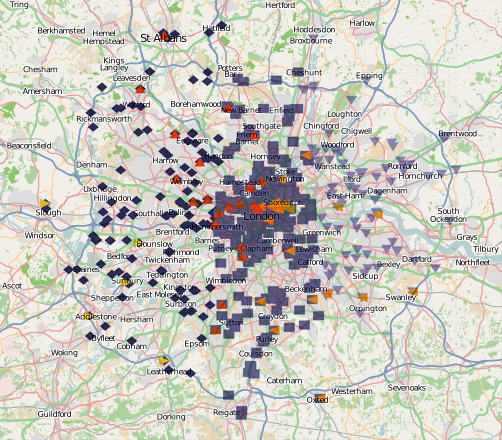
\includegraphics{images/futurework/map_london.jpg}
\caption{Results for clusters at timeslice 9:00 - 10:00am.}
\label{fig:clusters}
\end{figure}

In the above image, we can see a representation of the static clusters and the
timeslice clusters created from tweets. The static clusters were created for
all days for the timeframe of 9:00 - 10:00am, and the slice clusters are
created for the same time at the 29th of February 2012. In the image the three
clusters with tones of blue are the static clusters, and the three clusters
with tones of orange are the timeslice clusters.

The clusters are named from Static 1 to Static 3 and Slice cluster 1 to Slice
cluster 3 from left to right. The K-L divergence gave the following results:

\begin{center}
    \begin{tabular}{| l | l | l | l |}
    \hline
    & Slice cluster 1 & Slice cluster 2 & Slice cluster 3 \\ \hline
    Static 1 & 0.631128807559 & 0.309354831342 & 0.626666260517 \\ \hline
    Static 2 & -0.277093691689 & -0.598627406567 & -0.281078383944 \\ \hline
    Static 3 & -0.0722968487598 & -0.394347406928 & -0.0772419848337 \\ \hline
    \end{tabular}
\end{center}

Given these results we can consider that slice cluster 1 and 3 fall in the
normal behaviour of static cluster 3, but slice cluster 2 seems to suggest a
different behaviour from the static clusters and so could mean a rare event.
If our data were only about traffic could suggest a traffic accident for
example, and this is how it can be used in the future.

\subsection{Gamification}

\subsection{Further enhanced on the classification}
There are multiple ways that can improve the classifier. However, because of the strictly deadline of the project the time wasn�t enough to test all the possible improvements. Therefore the team decided to focus on the other parts of the project. One way to improve classification performance is to combine several classifiers. This can be easily be done by letting the multiple classifiers to use voting, and choose whichever label gets the most votes. For this style of voting, it's best to have an odd number of classifiers so that there are no ties. The individual classifiers should also use different algorithms. For example the Na�ve Bayes, the SVM and another classifier e.g a Decision Tree classifier can vote for a tweet and an algorithm can be used in order to classify the tweet accordingly.  Another way to enhance the classifier is to manually label more data and train the classifier from the beginning. Finally, the inclusion of trigrams collocations could increase the accuracy of the classification.  

\subsection{Analysis of other sources}
As the aim of this project is providing information to the user about traffic disruptions, more sources can 
easily be used for acquiring more information about disruptions in London and other areas. Such examples 
of sources would be news reports published in various websites. These reports could include accidents, general traffic or even 
bad road conditions due to the weather. Moreover, there exist TfL Twitter bots that frequently tweet
about traffic disruptions. Another source that can be used is Facebook. Data regarding traffic can be
extracted from posts, comments or even public groups whose current location is London.

\subsection{Enhanced geocoding}
Various methods exist that can improve the geocoding system implemented in our project. One technique, is extending the geocoding algorithm to recognise tweets written in languages other than English. In addition, advanced regular expressions can be added for extracting street addresses from tweets with a specific or wide range of formats. A more advanced geocoding system could also be implemented using classifiers. These classifiers can be trained with local addresses and be used to resolve locations from complex tweets. More classifiers can be created firstly to detect the language of the tweet and secondly to extract its location context that will be used to retrieve latitude and longitude points.
